\chapter{Decorator Pattern}

\section{Định nghĩa}
Decorator pattern là một trong những Pattern thuộc nhóm cấu trúc (Structural Pattern). Nó cho phép người dùng thêm chức năng mới vào đối tượng hiện tại mà không muốn ảnh hưởng đến các đối tượng khác. Kiểu thiết kế này có cấu trúc hoạt động như một lớp bao bọc (wrap) cho lớp hiện có. Mỗi khi cần thêm tính năng mới, đối tượng hiện có được wrap trong một đối tượng mới (decorator class).\\

Decorator pattern sử dụng composition thay vì inheritance (thừa kế) để mở rộng đối tượng. Decorator pattern còn được gọi là Wrapper hay Smart Proxy.

\section{Mục đích sử dụng}
Mục đích và lợi ích:
\begin{itemize}
	\item Tăng cường khả năng mở rộng của đối tượng, bởi vì những thay đổi được thực hiện bằng cách implement trên các lớp mới.
	\item Client sẽ không nhận thấy sự khác biệt khi bạn đưa cho nó một wrapper thay vì đối tượng gốc.
	\item Một đối tượng có thể được bao bọc bởi nhiều wrapper cùng một lúc.
	\item Cho phép thêm hoặc xóa tính năng của một đối tượng lúc thực thi (run-time).
\end{itemize}

\section{Mô hình cấu trúc}
\begin{center}
	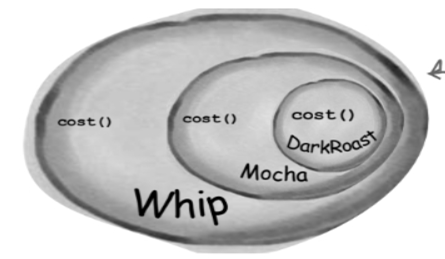
\includegraphics{GALLEYS/images/chapter4/diagram1}\\
\end{center}
\begin{center}
	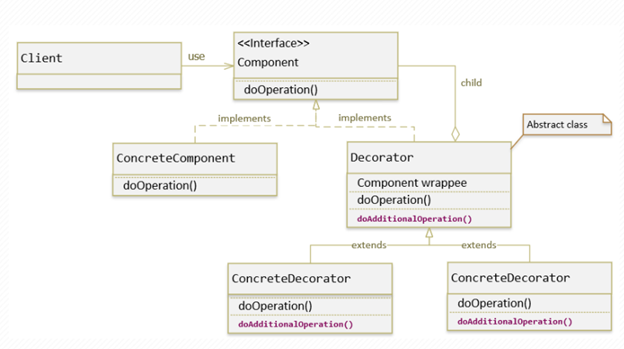
\includegraphics{GALLEYS/images/chapter4/diagram2}\\
\end{center}
Các thành phần trong mẫu thiết kế Decorator:\\
\textbf{Component} : là một interface quy định các method chung cần phải có cho tất cả các thành phần tham gia vào mẫu này.\\
\textbf{ConcreteComponent } : là lớp hiện thực (implements) các phương thức của Component.\\
\textbf{Decorator} : là một abstract class dùng để duy trì một tham chiếu của đối tượng Component và đồng thời cài đặt các phương thức của Component  interface.\\
\textbf{ConcreteDecorator } : là lớp hiện thực (implements) các phương thức của Decorator, nó cài đặt thêm các tính năng mới cho Component.\\
\textbf{Client} : đối tượng sử dụng Component.\\
VD:\\

Tình huống đặt ra trong quán cafee Starbuzz, giúp quản lí các loại đồ uống.\\
Khởi đầu là một lớp đồ uống :\\
\begin{multicols}{2}
	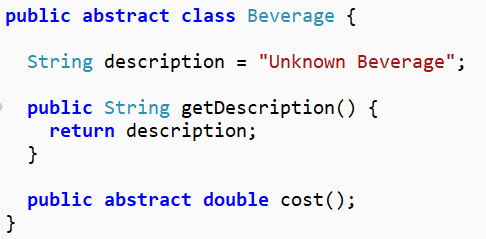
\includegraphics[width=1\columnwidth]{GALLEYS/images/chapter4/images1}\\
	
	Beverage là một lớp trừu tượng với một biến String description và hai phương thức trừu tượng getDescription() lấy ra thông tin đồ uống và cost() lấy ra giá của đồ uống.\\
	
	Lớp Beverage khá là đơn giản, nhưng đây là lớp cha của tất cả các lớp đồ uống – mọi lớp con đều phải extends từ đây.
	
\end{multicols}
\begin{center}
	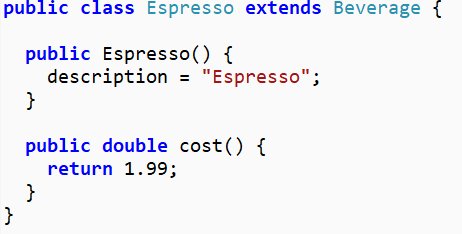
\includegraphics{GALLEYS/images/chapter4/images3}
\end{center}
Lớp cà phê Espresso có một construct khởi tạo thông tin là tên của loại cafee này và giá tiền là 1.99. 
Chúng ta sẽ tìm hiểu thêm một số loại sản phẩm khác:
\begin{multicols}{2}
	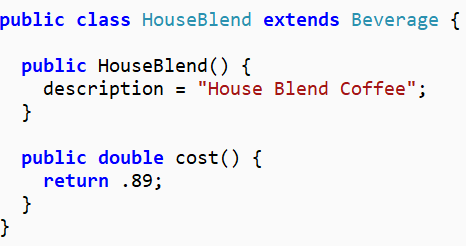
\includegraphics[width=0.9\columnwidth]{GALLEYS/images/chapter4/images4}
	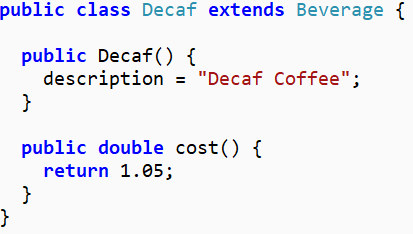
\includegraphics[width=0.9\columnwidth]{GALLEYS/images/chapter4/images5}
\end{multicols}
\begin{center}
	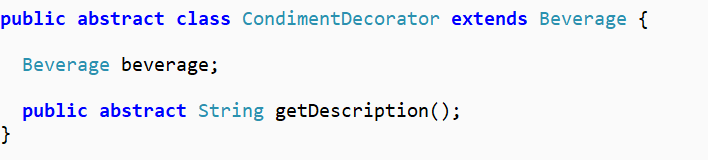
\includegraphics{GALLEYS/images/chapter4/images2}
\end{center}
Đây là lớp gia vị, nó phải kế thừa từ lớp đồ uống, ở đây có một phương thức trừu tượng getDescription() mô tả thông tin của gia vị.\\
Ở đây có 1 biến beverage và một lớp trừu tượng getDescription().
Nếu muốn một đồ uống nào đó có thêm gia vị , lớp đồ uống đó sẽ cần extends lại lớp này.

Như vậy có vẻ các lớp cơ sở khá là đầy đủ, chúng ta sẽ tiến hành đi sâu hơn vào các lớp con của chúng:\\
Lớp Espresso:\\

\begin{multicols}{2}
	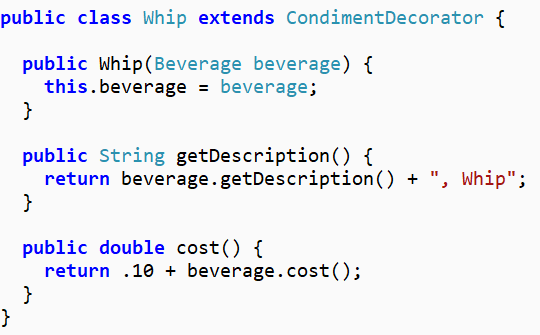
\includegraphics[width=0.9\columnwidth]{GALLEYS/images/chapter4/images6}
	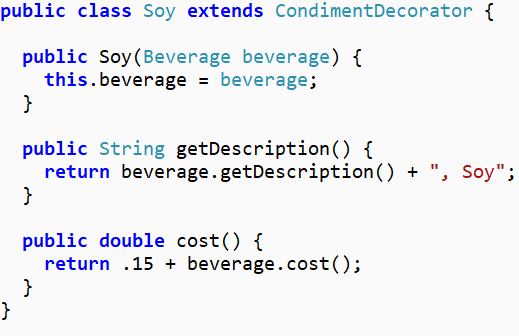
\includegraphics[width=0.9\columnwidth]{GALLEYS/images/chapter4/images7}
\end{multicols}

Điều thú vị ở đây là lớp nước uống có thêm gia vị này giá tiền sẽ được cộng thêm với giá cơ sở cho nước đó. Nó giảm độ phức tạp tính toán của nhà hàng.\\
Và đây là kết quả:
\begin{center}
	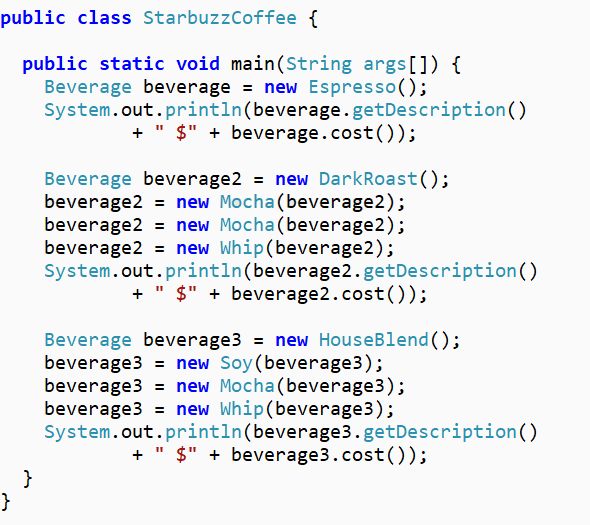
\includegraphics{GALLEYS/images/chapter4/images8}
	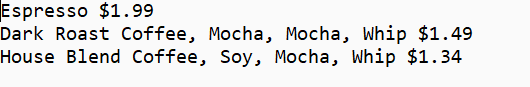
\includegraphics{GALLEYS/images/chapter4/images9}
\end{center}tế

\section{Decorator Pattern trong thực tế}
Decorator Pattern được áp dụng khi:

\begin{itemize}
	\item Khi muốn thêm tính năng mới cho các đối tượng mà không ảnh hưởng đến các đối tượng này.
	\item Khi không thể mở rộng một đối tượng bằng cách thừa kế (inheritance). Chẳng hạn, một class sử dụng từ khóa final, muốn mở rộng class này chỉ còn cách duy nhất là sử dụng decorator.
	\item Trong một số nhiều trường hợp mà việc sử dụng kế thừa sẽ mất nhiều công sức trong việc viết code. Ví dụ trên là một trong những trường hợp như vậy.
\end{itemize}
